% Judul dokumen
\title{Buku Tugas Akhir}
\author{Jabalnur}

% Pengaturan ukuran teks dan bentuk halaman dua sisi
\documentclass[12pt,twoside]{report}

% Pengaturan ukuran halaman dan margin
\usepackage[a4paper,top=30mm,left=30mm,right=20mm,bottom=25mm]{geometry}

% Pengaturan ukuran spasi
\usepackage[singlespacing]{setspace}
% \usepackage{tocloft}

% Pengaturan detail pada file PDF
\usepackage[pdfauthor={\@author},bookmarksnumbered,pdfborder={0 0 0}]{hyperref}

% Pengaturan jenis karakter
\usepackage[utf8]{inputenc}

% Pengaturan pewarnaan
\usepackage[table,xcdraw]{xcolor}

% Pengaturan kutipan artikel
\usepackage[style=apa, backend=biber]{biblatex}

% Package lainnya
\usepackage{changepage}
\usepackage{enumitem}
\usepackage{eso-pic}
\usepackage{txfonts} % Font times
% \usepackage{fontspec}
\usepackage{etoolbox}
\usepackage{graphicx}
\usepackage{lipsum}
\usepackage{longtable}
\usepackage{tabularx}
\usepackage{wrapfig}
\usepackage{float}
\usepackage{titlesec}
\usepackage{titletoc}

% Definisi untuk "Hati ini sengaja dikosongkan"
\patchcmd{\cleardoublepage}{\hbox{}}{
  \thispagestyle{empty}
  \vspace*{\fill}
  \begin{center}\textit{[Halaman ini sengaja dikosongkan]}\end{center}
  \vfill}{}{}

% Pengaturan Font
% \setmainfont{Trebuchet MS}

% Pengaturan penomoran halaman
\usepackage{fancyhdr}
\fancyhf{}
\renewcommand{\headrulewidth}{0pt}
\pagestyle{fancy}
\fancyfoot[LE,RO]{\thepage}
\patchcmd{\chapter}{plain}{fancy}{}{}
\patchcmd{\chapter}{empty}{plain}{}{}

% Command untuk bulan
\newcommand{\MONTH}{%
  \ifcase\the\month
  \or Januari% 1
  \or Februari% 2
  \or Maret% 3
  \or April% 4
  \or Mei% 5
  \or Juni% 6
  \or Juli% 7
  \or Agustus% 8
  \or September% 9
  \or Oktober% 10
  \or November% 11
  \or Desember% 12
  \fi}
\newcommand{\ENGMONTH}{%
  \ifcase\the\month
  \or January% 1
  \or February% 2
  \or March% 3
  \or April% 4
  \or May% 5
  \or June% 6
  \or July% 7
  \or August% 8
  \or September% 9
  \or October% 10
  \or November% 11
  \or December% 12
  \fi}

% Pengaturan format judul bab
\usepackage{titlesec}
\titleformat{\chapter}[display]{\bfseries\large}{BAB \centering\Roman{chapter}}{0ex}{\vspace{0ex}\centering}
\titleformat{\section}{\bfseries\large}{\MakeUppercase{\thesection}}{1ex}{\vspace{1ex}}
\titleformat{\subsection}{\bfseries\large}{\MakeUppercase{\thesubsection}}{1ex}{}
\titleformat{\subsubsection}{\bfseries\large}{\MakeUppercase{\thesubsubsection}}{1ex}{}
\titlespacing{\chapter}{0ex}{0ex}{4ex}
\titlespacing{\section}{0ex}{1ex}{0ex}
\titlespacing{\subsection}{0ex}{0.5ex}{0ex}
\titlespacing{\subsubsection}{0ex}{0.5ex}{0ex}

% Atur variabel berikut sesuai namanya

% nama
\newcommand{\name}{Jabalnur, S.T.}
\newcommand{\authorname}{Jabalnur, S.T.}
\newcommand{\nickname}{Jibi}
\newcommand{\advisor}{Agus Budi Raharjo, S.Kom, M.Kom., Ph.D.}
\newcommand{\examinerone}{None, S.T., M.Sc}
\newcommand{\examinertwo}{None, S.T., M.Sc}
\newcommand{\examinerthree}{None, ST., MT}
\newcommand{\headofdepartment}{Prof. Dr. Eng. Chastine Fatichah, S.Kom., M.Kom.}

% identitas
\newcommand{\nrp}{5025201241}
\newcommand{\advisornip}{1990202011022}
\newcommand{\examineronenip}{None}
\newcommand{\examinertwonip}{None}
\newcommand{\examinerthreenip}{None}
\newcommand{\headofdepartmentnip}{197512202001122002}

% judul
\newcommand{\tatitle}{\emph{INFLUENCE DEBUGGING AND TEST INPUT GENERATION}}
\newcommand{\engtatitle}{\emph{INFLUENCE DEBUGGING AND TEST INPUT GENERATION}}

% tempat
\newcommand{\place}{Surabaya}

% jurusan
\newcommand{\studyprogram}{Teknik Informatika}
\newcommand{\engstudyprogram}{Informatics Engineering}

% fakultas
\newcommand{\faculty}{Teknologi Elektro dan Informatika Cerdas}
\newcommand{\engfaculty}{Intelligent Electrical and Informatics Technology}

% singkatan fakultas
\newcommand{\facultyshort}{FTEIC}
\newcommand{\engfacultyshort}{F-ELECTICS}

% departemen
\newcommand{\department}{Teknik Informatika}
\newcommand{\engdepartment}{Informatics Engineering}

% kode mata kuliah
\newcommand{\coursecode}{EF234704}


% Tambahkan format tanda hubung yang benar di sini
\hyphenation{
  ro-ket
  me-ngem-bang-kan
  per-hi-tu-ngan
  tek-no-lo-gi
  me-la-ku-kan
  ber-so-si-al-i-sa-si
}

% Menambahkan resource daftar pustaka
\addbibresource{pustaka/pustaka.bib}

% Pengaturan format potongan kode
\usepackage{listings}
\definecolor{comment}{RGB}{0,128,0}
\definecolor{string}{RGB}{255,0,0}
\definecolor{keyword}{RGB}{0,0,255}
\lstdefinestyle{codestyle}{
  commentstyle=\color{comment},
  stringstyle=\color{string},
  keywordstyle=\color{keyword},
  basicstyle=\footnotesize\ttfamily,
  numbers=left,
  numberstyle=\tiny,
  numbersep=5pt,
  frame=lines,
  breaklines=true,
  prebreak=\raisebox{0ex}[0ex][0ex]{\ensuremath{\hookleftarrow}},
  showstringspaces=false,
  upquote=true,
  tabsize=2,
}
\lstset{style=codestyle}

% Pengaturan format daftar isi
\titlecontents{chapter}
[4.5em]
{\smallskip}
{\contentslabel[\MakeUppercase{bab~\romannumeral\thecontentslabel}]{4em}\MakeUppercase}
{\hspace*{-4em}\MakeUppercase}
{\hfill\contentspage}[\medskip]

% Isi keseluruhan dokumen
\begin{document}

% Sampul luar Bahasa Indonesia
\newcommand\covercontents{sampul/konten-id.tex}
\AddToShipoutPictureBG*{
  \AtPageLowerLeft{
    % Ubah nilai berikut jika posisi horizontal background tidak sesuai
    \hspace{-3.25mm}

    % Ubah nilai berikut jika posisi vertikal background tidak sesuai
    \raisebox{0mm}{
      
\includegraphics[width=\paperwidth,height=\paperheight]{sampul/gambar/sampul-luar.png}
    }
  }
}

% Menyembunyikan nomor halaman
\thispagestyle{empty}

% Pengaturan margin untuk menyesuaikan konten sampul
\newgeometry{
  top=55mm,
  left=30mm,
  right=20mm,
  bottom=20mm
}

\begin{flushleft}

  % Pemilihan font sans serif
  \sffamily

  % Pemilihan warna font putih
  \color{white}

  % Pemilihan font bold
  \fontseries{bx}
  \selectfont
  \begin{spacing}{1.5}
    \input{\covercontents}
  \end{spacing}

\end{flushleft}

\restoregeometry


% Atur ulang penomoran halaman
\setcounter{page}{1}

% Sampul dalam Bahasa Indonesia
\renewcommand\covercontents{sampul/konten-id.tex}
\AddToShipoutPictureBG*{
  \AtPageLowerLeft{
    % Ubah nilai berikut jika posisi horizontal background tidak sesuai
    \hspace{-4mm}

    % Ubah nilai berikut jika posisi vertikal background tidak sesuai
    \raisebox{0mm}{
      
\includegraphics[width=\paperwidth,height=\paperheight]{sampul/gambar/sampul-luar-tipis.png}
    }
  }
}

% Menyembunyikan nomor halaman
\thispagestyle{empty}

% Pengaturan margin untuk menyesuaikan konten sampul
\newgeometry{
  top=65mm,
  left=30mm,
  right=30mm,
  bottom=20mm
}

\begin{flushleft}

  % Pemilihan font sans serif
  \sffamily

  % Pemilihan font bold
  \fontseries{bx}
  \selectfont
  \begin{spacing}{1.5}
    \input{\covercontents}
  \end{spacing}

\end{flushleft}

\restoregeometry

\clearpage
\cleardoublepage

% Sampul dalam Bahasa Inggris
\renewcommand\covercontents{sampul/konten-en.tex}
\AddToShipoutPictureBG*{
  \AtPageLowerLeft{
    % Ubah nilai berikut jika posisi horizontal background tidak sesuai
    \hspace{-4mm}

    % Ubah nilai berikut jika posisi vertikal background tidak sesuai
    \raisebox{0mm}{
      
\includegraphics[width=\paperwidth,height=\paperheight]{sampul/gambar/sampul-luar-tipis.png}
    }
  }
}

% Menyembunyikan nomor halaman
\thispagestyle{empty}

% Pengaturan margin untuk menyesuaikan konten sampul
\newgeometry{
  top=65mm,
  left=30mm,
  right=30mm,
  bottom=20mm
}

\begin{flushleft}

  % Pemilihan font sans serif
  \sffamily

  % Pemilihan font bold
  \fontseries{bx}
  \selectfont
  \begin{spacing}{1.5}
    \input{\covercontents}
  \end{spacing}

\end{flushleft}

\restoregeometry

\cleardoublepage

% Label tabel dan gambar dalam bahasa indonesia
\renewcommand{\figurename}{Gambar}
\renewcommand{\tablename}{Tabel}

% Pengaturan ukuran indentasi paragraf
\setlength{\parindent}{2em}

% Pengaturan ukuran spasi paragraf
\setlength{\parskip}{1ex}

% Lembar pengesahan
\chapter*{LEMBAR PENGESAHAN}
\addcontentsline{toc}{chapter}{LEMBAR PENGESAHAN}

% Menyembunyikan nomor halaman
\begin{center}
  \textbf{\tatitle{}}
\end{center}

\begingroup
% Pemilihan font ukuran small
\small

\begin{center}
  \textbf{TUGAS AKHIR}
  \\Diajukan untuk memenuhi salah satu syarat \\
  memperoleh gelar Sarjana Teknik pada \\
  Program Studi S-1 \studyprogram{} \\
  Departemen \department{} \\
  Fakultas \faculty{} \\
  Institut Teknologi Sepuluh Nopember
\end{center}

\begin{center}
  Oleh: \textbf{\name{}}
  \\NRP. \nrp{}
\end{center}

\begin{center}
  Disetujui oleh Tim Penguji Tugas Akhir:
\end{center}

\begingroup
% Menghilangkan padding
\setlength{\tabcolsep}{0pt}

\noindent
\begin{tabularx}{\textwidth}{X l}
  \advisor{}               & (Pembimbing I)                      \\
  NIP: \advisornip{}       &                                     \\
                           & ................................... \\
                           &                                     \\
                           &                                     \\
  \examinerone{}.          & (Penguji I)                         \\
  NIP: \examineronenip{}   &                                     \\
                           & ................................... \\
                           &                                     \\
                           &                                     \\
  \examinertwo{}.          & (Penguji II)                        \\
  NIP: \examinertwonip{}   &                                     \\
                           & ................................... \\
                           &                                     \\
                           &                                     \\
\end{tabularx}
\endgroup

\begin{center}
  Mengetahui, \\
  Kepala Departemen \department{} \facultyshort{} - ITS\\

  \vspace{8ex}

  \underline{\headofdepartment{}.} \\
  NIP. \headofdepartmentnip{}
\end{center}

\begin{center}
  \textbf{\MakeUppercase{\place{}}\\\MONTH{}, \the\year{}}
\end{center}
\endgroup

\thispagestyle{empty}
\begin{tikzpicture}[remember picture, overlay]
  \node[anchor=north west, inner sep=0] at (current page.north west) {
      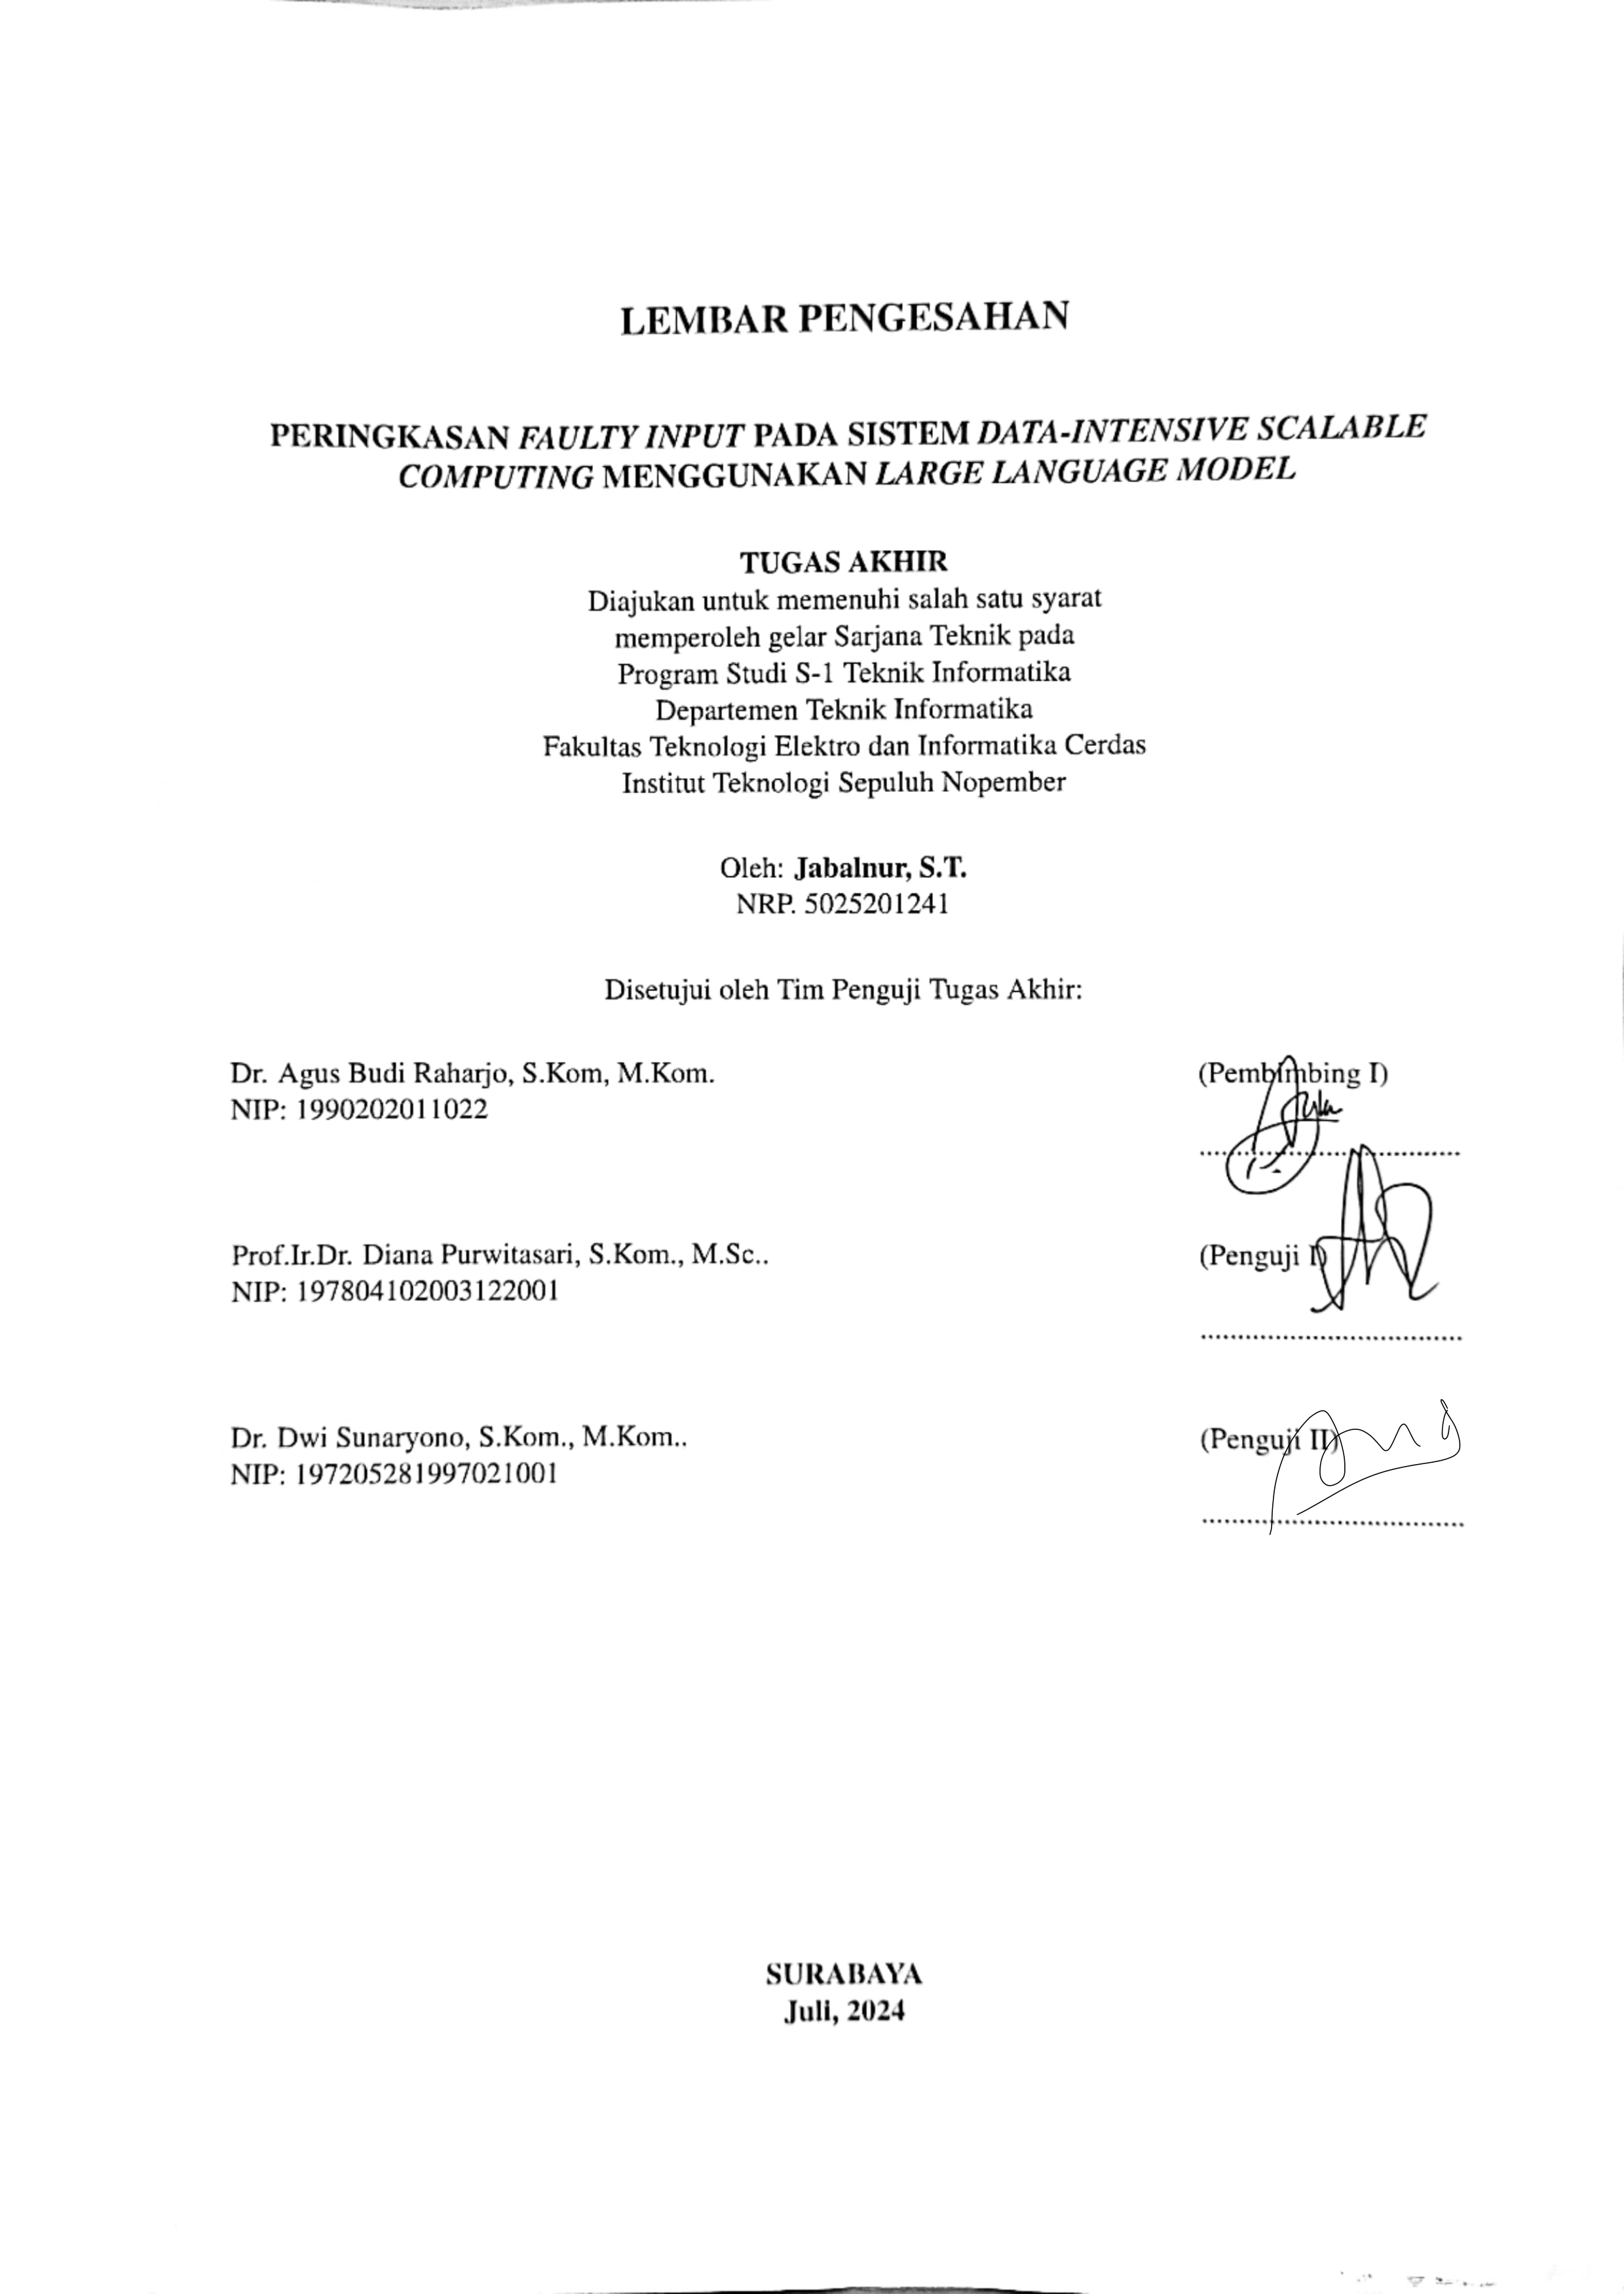
\includegraphics[width=\paperwidth, height=\paperheight]{gambar/LembarPengesahanIndo.png}
  };
\end{tikzpicture}

\cleardoublepage
\begin{center}
  \large
  \textbf{APPROVAL SHEET}
\end{center}

% Menyembunyikan nomor halaman
\thispagestyle{empty}

\begin{center}
  \textbf{\engtatitle{}}
\end{center}

\begingroup
% Pemilihan font ukuran small
\small

\begin{center}
  \textbf{FINAL PROJECT}
  \\Submitted to fulfill one of the requirements \\
  for obtaining a degree Bachelor of Engineering at \\
  Undergraduate Study Program of \engstudyprogram{} \\
  Department of \engdepartment{} \\
  Faculty of \engfaculty{} \\
  Sepuluh Nopember Institute of Technology
\end{center}

\begin{center}
  By: \textbf{\name{}}
  \\NRP. \nrp{}
\end{center}

\begin{center}
  Approved by Final Project Examiner Team:
\end{center}

\begingroup
% Menghilangkan padding
\setlength{\tabcolsep}{0pt}

\noindent
\begin{tabularx}{\textwidth}{X l}
  \advisor{}               & (Advisor I)                         \\
  NIP: \advisornip{}       &                                     \\
                           & ................................... \\
                           &                                     \\
                           &                                     \\
  \coadvisor{}             & (Co-Advisor II)                     \\
  NIP: \coadvisornip{}     &                                     \\
                           & ................................... \\
                           &                                     \\
                           &                                     \\
  \examinerone{}.          & (Examiner I)                        \\
  NIP: \examineronenip{}   &                                     \\
                           & ................................... \\
                           &                                     \\
                           &                                     \\
  \examinertwo{}.          & (Examiner II)                       \\
  NIP: \examinertwonip{}   &                                     \\
                           & ................................... \\
                           &                                     \\
                           &                                     \\
  \examinerthree{}.        & (Examiner III)                      \\
  NIP: \examinerthreenip{} &                                     \\
                           & ................................... \\
\end{tabularx}
\endgroup


\begin{center}
  Acknowledged, \\
  Head of \engdepartment{} Department \engfacultyshort{} - ITS \\

  \vspace{8ex}

  \underline{\headofdepartment{}.} \\
  NIP. \headofdepartmentnip{}
\end{center}

\begin{center}
  \textbf{\MakeUppercase{\place{}}\\\ENGMONTH{}, \the\year{}}
\end{center}
\endgroup

\cleardoublepage

% Pernyataan keaslian
\chapter*{PERNYATAAN ORISINALITAS}
\addcontentsline{toc}{chapter}{PERNYATAAN ORISINALITAS}

% Menyembunyikan nomor halaman
\thispagestyle{empty}

\vspace{2ex}

% Ubah paragraf-paragraf berikut sesuai dengan yang ingin diisi pada pernyataan keaslian

\noindent Yang bertanda tangan dibawah ini:

\noindent\begin{tabularx}{\textwidth}{l l X}
                         &   &                            \\
  Nama Mahasiswa / NRP   & : & \name{} / \nrp{}           \\
  Departemen             & : & \department{}              \\
  Dosen Pembimbing / NIP & : & \advisor{} / \advisornip{} \\
                         &   &                            \\
\end{tabularx}

Dengan ini menyatakan bahwa Tugas Akhir dengan judul "\tatitle{}" adalah hasil karya sendiri, berfsifat orisinal, dan ditulis dengan mengikuti kaidah penulisan ilmiah.

Bilamana di kemudian hari ditemukan ketidaksesuaian dengan pernyataan ini, maka saya bersedia menerima sanksi sesuai dengan ketentuan yang berlaku di Institut Teknologi Sepuluh Nopember.

\vspace{8ex}

\noindent\begin{tabularx}{\textwidth}{X l}
                     & \place{}, \ENGMONTH{} \the\year{} \\
                     &                                   \\
  Mengetahui         &                                   \\
  Dosen Pembimbing   & Mahasiswa                         \\
                     &                                   \\
                     &                                   \\
                     &                                   \\
                     &                                   \\
                     &                                   \\
  \advisor{}         & \name{}                           \\
  NIP. \advisornip{} & NRP. \nrp{}                       \\
\end{tabularx}

\cleardoublepage
\begin{center}
  \large
  \textbf{STATEMENT OF ORIGINALITY}
\end{center}

% Menyembunyikan nomor halaman
\thispagestyle{empty}

\vspace{2ex}

% Ubah paragraf-paragraf berikut sesuai dengan yang ingin diisi pada pernyataan keaslian

\noindent The undersigned below:

\noindent\begin{tabularx}{\textwidth}{l l X}
                        &   &                            \\
  Name of student / NRP & : & \name{} / \nrp{}           \\
  Department            & : & \engdepartment{}           \\
  Advisor / NIP         & : & \advisor{} / \advisornip{} \\
                        &   &                            \\
\end{tabularx}

Hereby declared that the Final Project with the title of "\engtatitle{}" is the result of my own work, is original, and is written by following the rules of scientific writing.

If in future there is a discrepancy with this statement, then I am willing to accept sanctions in accordance with provisions that apply at Sepuluh Nopember Institute of Technology.

\vspace{8ex}

\noindent\begin{tabularx}{\textwidth}{X l}
                     & \place{}, \ENGMONTH{} \the\year{} \\
                     &                                   \\
  Acknowledged       &                                   \\
  Advisor            & Student                           \\
                     &                                   \\
                     &                                   \\
                     &                                   \\
                     &                                   \\
                     &                                   \\
  \advisor{}         & \name{}                           \\
  NIP. \advisornip{} & NRP. \nrp{}                       \\
\end{tabularx}

\begin{tikzpicture}[remember picture, overlay]
  \node[anchor=north west, inner sep=0] at (current page.north west) {
      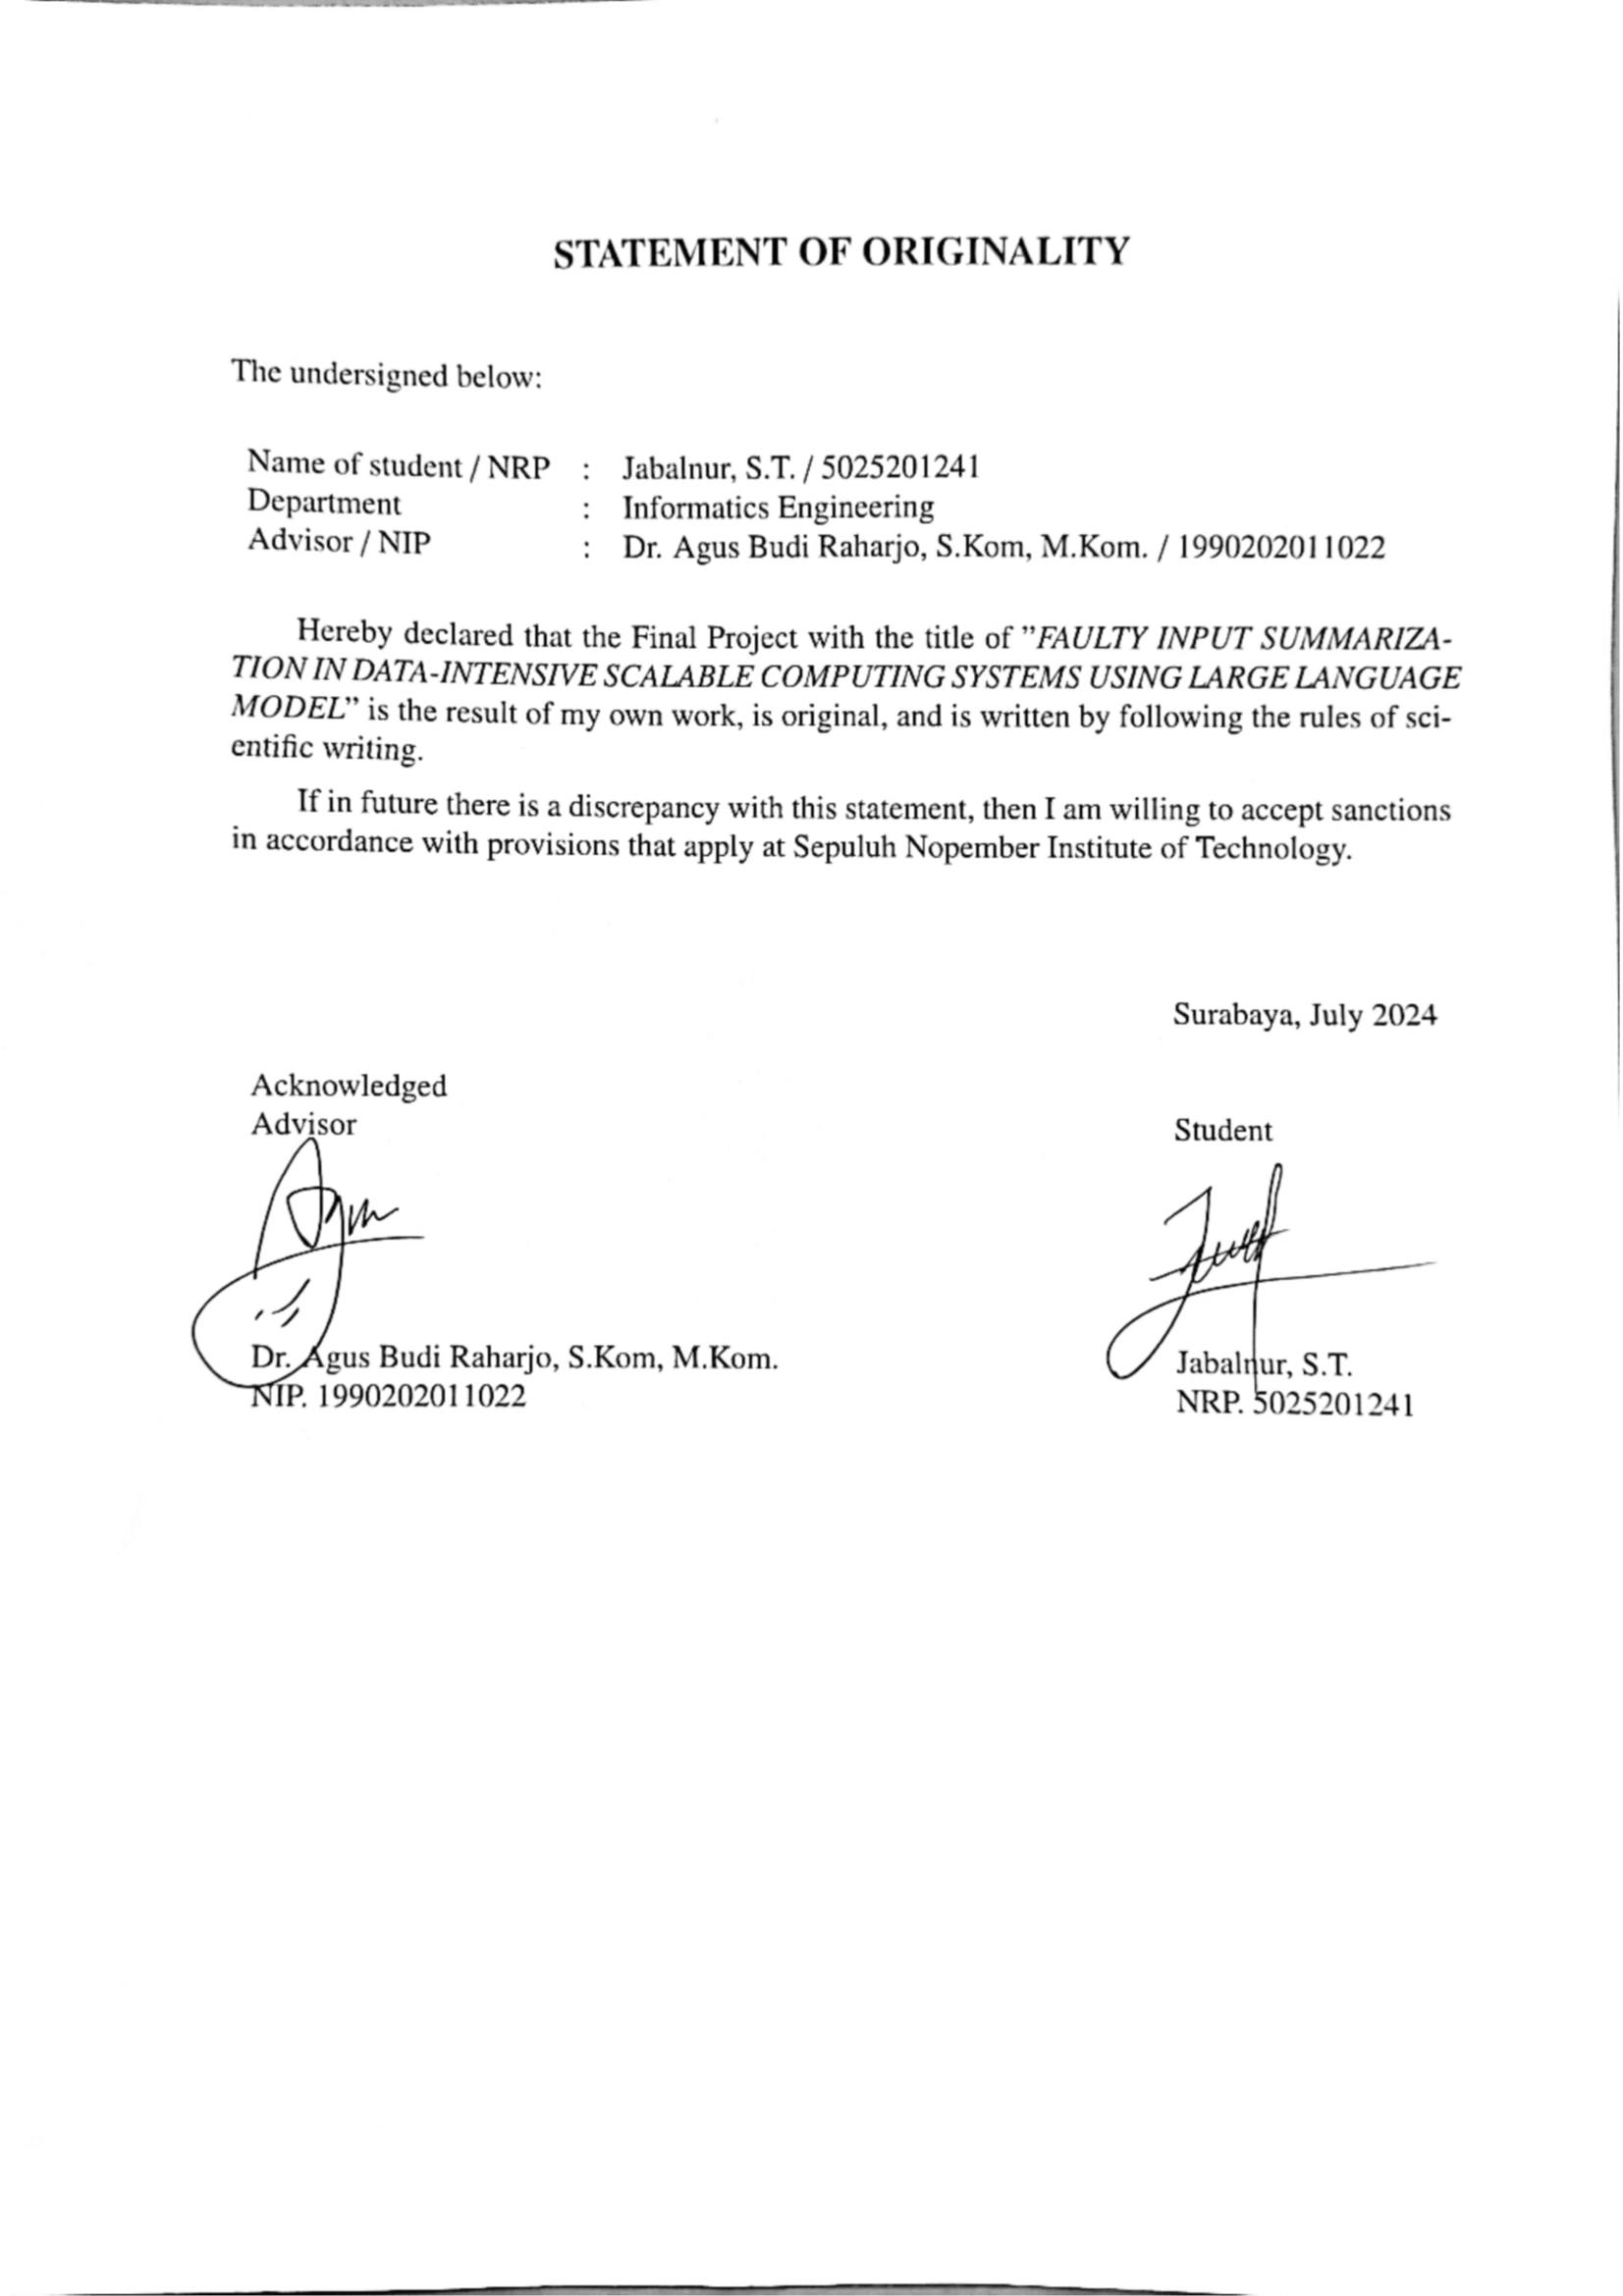
\includegraphics[width=\paperwidth, height=\paperheight]{gambar/PernyataanOrisinalitasEng.png}
  };
\end{tikzpicture}
\cleardoublepage

% Nomor halaman pembuka dimulai dari sini
\pagenumbering{roman}

% Abstrak Bahasa Indonesia
\chapter*{ABSTRAK}
\addcontentsline{toc}{chapter}{ABSTRAK}

\vspace{2ex}

\begingroup
% Menghilangkan padding
\setlength{\tabcolsep}{0pt}

\noindent
\begin{tabularx}{\textwidth}{l >{\centering}m{2em} X}
  Nama Mahasiswa    & : & \name{}         \\

  Judul Tugas Akhir & : & \tatitle{}      \\

  Pembimbing        & : & 1. \advisor{}   \\
\end{tabularx}
\endgroup

% Ubah paragraf berikut dengan abstrak dari tugas akhir
% Framework pemrosesan data skala besar seperti \textit{Apache Spark} telah memungkinkan \textit{developer} untuk memproses petabyte data dengan aplikasi \textit{Data-Intensive Scalable Computing (DISC)}. Seperti halnya perangkat lunak lainnya, kesalahan dalam aplikasi \textit{DISC} adalah hal yang umum. Kesalahan tersebut dapat timbul karena dataset input yang tidak bersih atau implementasi aplikasi, yang membuat \textit{developer} harus mengidentifikasi akar penyebab di antara miliaran data input. Proses \textit{Data Provenance} dan \textit{debugging} otomatis memerlukan instrumentasi aplikasi \textit{DISC} atau melakukan \textit{search-based fault isolation} yang memakan banyak sumber daya.

% Penelitian ini bertujuan untuk menunjukkan potensi penggunaan \textit{language model} untuk menghasilkan dataset input minimal namun dapat mereproduksi kesalahan yang sama seperti yang diamati pada data masukan skala besar aslinya. Kami membuat \textit{FISUM} (\textit{Fault-inducing Inputs Summarization}), yang melatih model dengan \textit{faulty input} secara historis untuk menghasilkan baris salah baru yang minimal. \textit{FISUM} menggunakan \textit{Data Provenance Engine} yang dibangun untuk \textit{Apache Spark}, untuk memulihkan input yang menyebabkan kesalahan. Kemudian melatih sebuah \textit{lightweight language model}, \textit{DistilGPT}, menggunakan input yang menyebabkan kegagalan ini untuk menghasilkan input minimal yang mengungkapkan kesalahan yang sama.

% Pada percobaan dengan aplikasi \textit{DISC} bermasalah yang telah ada, bahkan dengan model ringan, \textit{FISUM} secara efektif dapat merangkum input yang menyebabkan kesalahan, mengurangi input asli dari alat \textit{data provenance} sebesar 99\%, namun masih dapat menyebabkan kesalahan yang sama. \textit{FISUM} menghasilkan \textit{faulty input} dalam waktu kurang dari 50 milidetik per baris, rata-rata.

Framework pemrosesan data skala besar seperti Apache Spark telah memungkinkan \textit{developer} untuk memproses petabyte data dengan aplikasi \textit{Data-Intensive Scalable Computing (DISC)}. Seperti halnya perangkat lunak lainnya, kesalahan dalam aplikasi DISC adalah hal yang umum. Kesalahan tersebut dapat timbul karena dataset input yang tidak bersih atau implementasi aplikasi, yang membuat \textit{developer} harus mengidentifikasi akar penyebab di antara miliaran data input. Proses \textit{Data Provenance} dan \textit{debugging} otomatis memerlukan instrumentasi aplikasi DISC atau melakukan \textit{search-based fault isolation} yang memakan banyak sumber daya. Penelitian ini bertujuan untuk menunjukkan potensi penggunaan \textit{language model} untuk menghasilkan dataset input minimal namun dapat mereproduksi kesalahan yang sama seperti yang diamati pada data masukan skala besar aslinya. Kami membuat FISUM (\textit{Fault-inducing Inputs Summarization}), yang melatih model dengan \textit{faulty input} secara historis untuk menghasilkan baris salah baru yang minimal dan memiliki karakteristik yang sama dengan data aslinya.

FISUM menggunakan Titian, sebuah \textit{Data Provenance Engine} yang dibangun untuk Apache Spark, untuk memulihkan input yang menyebabkan kesalahan. \textit{Data Provenance Engine} merupakan sebuah sistem yang melacak asal-usul, sejarah, dan perjalanan data dalam sebuah sistem komputasi untuk memudahkan dalam mengidentifikasi sumber kesalahan dan memahami transformasi data dari sumber aslinya hingga ke bentuk akhirnya. Titian kemudian ditanamkan ke dalam aplikasi DISC yang memiliki keluaran bermasalah untuk menemukan \textit{Faulty Input}, yaitu baris data pada dataset yang menjadi penyebab keluaran bermasalah pada aplikasi DISC. Sebuah \textit{lightweight language model}, DistilGPT2 milik HuggingFace \textit{Faulty Input} kemudian dilatih menggunakan dataset awal milik aplikasi DISC untuk membiasakan model tersebut dengan dataset aplikasi, kemudian model tersebut dilatih kembali dengan menggunakan \textit{Faulty Input} dari Titian untuk memahami karakteristik dari \textit{Faulty Input} tersebut. DistilGPT2 yang telah dilatih akhirnya dapat digunakan untuk menghasilkan \textit{Faulty Input} baru yang memiliki ukuran yang jauh lebih kecil dari ukuran aslinya dengan tetap mempertahankan kemiripan karakteristik kesalahan pada \textit{Faulty Input} awal dalam waktu yang cukup singkat.

Percobaan dilakukan dengan menguji 16 \textit{Benchmark Application} yang merupakan aplikasi DISC dengan menghitung tingkat akurasi FISUM dalam menemukan \textit{Faulty Input} pada dataset aplikasi, menghitung tingkat akurasi dari kesalahan yang dimiliki oleh \textit{Faulty Input} baru dan menghitung \textit{Mean Square Error (MSE)} dari karakteristik yang dimiliki oleh \textit{Faulty Input} awal dan baru. FISUM secara efektif dapat menemukan \textit{Faulty Input} pada aplikasi DISC dengan akurasi 100\%, dapat merangkum \textit{Faulty Input} dengan tingkat akurasi 99.4\% dalam waktu kurang dari 0.082 detik per baris, dan dapat menyajikan kemiripan karakteristik dari \textit{Faulty Input} awal dan baru dengan MSE sebesar 0.262.


% Ubah kata-kata berikut dengan kata kunci dari tugas akhir
Kata Kunci: \emph{Debugging}, \emph{Generative AI}, \emph{Faults}, \emph{Language Models}.

\cleardoublepage

% Abstrak Bahasa Inggris
\begin{center}
  \large\textbf{ABSTRACT}
\end{center}

\vspace{2ex}

\begingroup
% Menghilangkan padding
\setlength{\tabcolsep}{0pt}

\noindent
\begin{tabularx}{\textwidth}{l >{\centering}m{3em} X}
  \emph{Name}     & : & \name{}         \\

  \emph{Title}    & : & \engtatitle{}   \\

  \emph{Advisor}    & : & \advisor{}   \\

  \\
\end{tabularx}
\endgroup

% Ubah paragraf berikut dengan abstrak dari tugas akhir dalam Bahasa Inggris
\emph{Large-scale data processing frameworks like Apache Spark have enabled developers to process petabytes of data with Data-Intensive Scalable Computing (DISC) applications. Like any other software, faults in DISC applications are common. These faults can arise due to unclean input datasets or application implementation, requiring developers to identify the root cause among billions of input data. The process of Data Provenance and automated debugging requires instrumenting DISC applications or performing search-based fault isolation, which consumes significant resources.}

\emph{This study aims to demonstrate the potential use of language models to generate minimal input datasets capable of reproducing the same faults observed in the original large-scale input data. We introduce FISUM (Fault-inducing Inputs Summarization), which trains a model on historically faulty inputs to generate new minimal faulty rows. FISUM leverages the Data Provenance Engine built for Apache Spark to recover fault-inducing inputs. It then trains a lightweight language model, DistilGPT, on these failure-inducing inputs to generate minimal fault-revealing inputs.}

\emph{In experiments with existing faulty DISC applications, even with a lightweight model, FISUM effectively summarizes fault-inducing input, reducing the original input from the data provenance tool by 99\%, while still inducing the same fault. FISUM generates faulty inputs in under 50 milliseconds per row, on average.}

% Ubah kata-kata berikut dengan kata kunci dari tugas akhir dalam Bahasa Inggris
\emph{Keywords}: \emph{Debugging}, \emph{Generative AI}, \emph{Faults}, \emph{Language Models}.

\cleardoublepage

% Kata pengantar
\chapter*{KATA PENGANTAR}
\addcontentsline{toc}{chapter}{KATA PENGANTAR}

\vspace{2ex}

% Ubah paragraf-paragraf berikut dengan isi dari kata pengantar

Puji dan syukur penulis panjat kan kepada Tuhan yang Maha Esa atas
berkat, rahmat, dan karunia-Nya sehingga tugas akhir yang berjudul "\tatitle" dapat
diselesaikan dengan baik sebagai salah satu syarat dalam menyelesaikan Strata-1
pada Departemen \studyprogram{}, \faculty{}, \institute{}.

Penulis menyadari bahwa dalam penyusunan dan penulisan tugas akhir ini
tidak lepas dari bantuan, bimbingan, serta dukungan dari berbagai pihak, dari masa
perkuliahan hingga penyusunan tugas akhir. Oleh karena itu, penulis menyampaikan
terima kasih kepada:

\begin{enumerate}[nolistsep, noitemsep,topsep=0pt]

  \item Kedua orang tua penulis, Bapak Jamaluddin S, S.Pd., dan 
  Ibu Hj. Nurbaya Nur yang tidak pernah lelah dalam mendidik dan 
  memberikan dukungan, doa, serta semangat kepada penulis.

  \item Bapak \advisor{}, selaku Dosen Pembimbing I Tugas 
  Akhir penulis yang senantiasa membimbing
  dan menyediakan waktu, tenaga, dan perhatiannya di sepanjang 
  pengerjaan tugas akhir ini.

  \item Bapak Ali Gulzar, Ahmad, dan Gista yang telah memberikan
  bimbingan, arahan, bantuin selama pengerjaan tugas akhir ini.

  \item Bapak dan Ibu dari Direktorat Jenderal Pendidikan Tinggi
  Kementerian Pendidikan, Kebudayaan, Riset, dan Teknologi yang telah
  memberikan beasiswa LPDP yang telah membantu penulis dalam menyelesaikan
  tugas akhir ini.

  \item Segenap Dosen dan Tenaga Pendidik \department{} \faculty{} \institute{}
  yang telah banyak membantu semasa perkuliahan dan dalam penyelesaian tugas akhir.

  \item Saudara-saudara \emph{Backstreet} yang telah memberikan
  bantuan, semangat, waktu, serta segala macam hal yang telah membawa
  penulis hingga bisa menjadi seperti sekarang ini.

  \item Sahabat-sahabat dari Kontrakan KP IV No.5B yang telah memberikan
  dukungan, semangat, dan bantuan dalam menjalani perkuliahan ini.

  \item Teman-teman dari Kanda ITS yang telah memberikan dukungan, semangat,
  dan bantuan selama masa perkuliahan dan pengerjaan tugas akhir.

  \item Seluruh pihak yang tidak sempat tersebutkan dan tanpa sadar telah
  menjadi inspirasi serta banyak membantu penulis dalam menyelesaikan tugas akhir.

\end{enumerate}

Akhir kata, penulis menyadari bahwa tugas akhir ini mash jauh dari kata
sempurna, oleh karenanya diharapkan segala bentuk saran serta masukan yang
membangun dari berbagai pihak. Semoga tugas akhir ini dapat memberikan
sumbangsih dan manfaat besar bagi kehidupan manusia

\begin{flushright}
  \begin{tabular}[b]{c}
    \place{}, \MONTH{} \the\year{} \\
    \\
    \\
    \\
    \\
    \name{}
  \end{tabular}
\end{flushright}

\cleardoublepage

% Daftar isi
\renewcommand*\contentsname{DAFTAR ISI}
\label{chap:daftar isi}
\addcontentsline{toc}{chapter}{\contentsname}
\tableofcontents
\cleardoublepage

% Daftar gambar
\renewcommand*\listfigurename{DAFTAR GAMBAR}
\label{chap:daftar gambar}
\addcontentsline{toc}{chapter}{\listfigurename}
\listoffigures
\cleardoublepage

% Daftar tabel
\renewcommand*\listtablename{DAFTAR TABEL}
\label{chap:daftar tabel}
\addcontentsline{toc}{chapter}{\listtablename}
\listoftables
\cleardoublepage

% Nomor halaman isi dimulai dari sini
\pagenumbering{arabic}

% Bab 1 pendahuluan
\chapter{PENDAHULUAN}\label{chap:pendahuluan}

% Ubah bagian-bagian berikut dengan isi dari pendahuluan

\section{Latar Belakang}\label{sec:latarbelakang}

Analisis data modern memerlukan penanganan data berskala 
terabyte yang tersebar di berbagai mesin. Untuk membuat 
ini dapat dilakukan, kerangka kerja 
\emph{Data Intensive Scalable Computing (DISC)} seperti 
Apache Spark~\cite{zaharia2010,spark} dan 
Google MapReduce~\cite{dean2008} memungkinkan analis 
data untuk membuat aplikasi terdistribusi. Volume besar 
data input untuk aplikasi DISC, ditambah dengan sifat 
terdistribusi dari program, membuat debugging menjadi 
sangat menantang.
Bayangkan sebuah program yang menghitung rata-rata 
curah hujan per tahun di Amerika Serikat. Ini 
memerlukan penghitungan rata-rata dari puluhan 
juta nilai yang dikumpulkan dari sensor yang 
tersebar di seluruh negeri. Setelah menjalankan 
program, analis memperhatikan bahwa nilai rata-rata 
yang dihasilkan sangat tinggi dan mencurigakan. 
Bagaimana programmer akan mendiagnosis penyebab 
kesalahan ini?

Beberapa penelitian dalam debugging program telah 
berfokus pada pengurangan ukuran input yang 
menyebabkan kesalahan~\cite{zeller2002,misherghi2006,kirschner2020,clause2009}.
Banyak dari teknik ini 
adalah varian dari algoritma delta debugging, 
yang bekerja dengan menjalankan program berulang 
kali dengan segmen-segmen berbeda dari input yang 
menyebabkan kesalahan hingga algoritma tersebut 
menemukan ukuran input minimal. Teknik pengurangan 
input tradisional ini, meskipun telah dicoba~\cite{gulzar2018}, tidak 
dapat diterapkan pada aplikasi DISC karena memerlukan 
eksekusi berulang yang lambat dan memakan banyak 
sumber daya.

Dalam penelitian ini, kami mengusulkan teknik berbasis 
\emph{large language model} (LLM) yang efisien untuk 
merangkum data yang bermasalah, yang mungkin mencakup 
jutaan baris, menjadi hanya beberapa baris yang tetap 
dapat mereproduksi kesalahan. Kami mewujudkan ide ini 
dalam alat yang disebut FISUM, sebuah sistem 
\emph{Fault-inducing Inputs Summarization}. 
Inti dari teknik kami adalah bahwa LLM generatif 
modern dapat dilatih untuk menangkap pola input 
yang memicu kesalahan dari data besar. Hasil dari 
pelatihan model ini kemudian dapat digunakan untuk 
menghasilkan input baru yang menyebabkan pola 
kesalahan yang sama.

Teknik kami memerlukan proses \emph{pre-training} 
dari model GPT versi ringan, distilGPT, pada seluruh 
data input. Langkah \emph{unsupervised} ini 
memungkinkan model untuk mempelajari struktur 
dasar dan pola dari data tersebut. Kami kemudian 
menggunakan Titian~\cite{interlandi2015} untuk mengambil subset besar 
dari input yang dianggap mencurigakan terkait 
dengan eksekusi yang salah. distilGPT kemudian 
dilatih ulang pada data mencurigakan ini untuk 
membiasakannya dalam menghasilkan input yang 
menyebabkan kesalahan. Akhirnya, distilGPT diarahkan 
untuk menghasilkan data yang dapat mereproduksi 
kesalahan tersebut.
Untuk mengevaluasi teknik kami, kami menggunakan satu 
set program \emph{benchmark} dari penelitian sebelumnya 
tentang \emph{debugging} dan pengujian aplikasi 
DISC~\cite{gulzar2019,humayun2023,zhang2021}. 

\section{Rumusan Permasalahan}
\label{sec:permasalahan}

Berdasarkan latar belakang di atas, maka dapat ditarik rumusan masalah sebagai berikut:

\begin{enumerate}[nolistsep]

   \item Apakah input yang bermasalah yang dihasilkan oleh FISUM masih mempertahankan kemampuan deteksi kesalahan?

   \item Berapa banyak persentase pengurangan input bermasalah yang dapat dihasilkan oleh FISUM dari dataset yang diberikan?

   \item Berapa lama waktu yang dibutuhkan untuk menghasilkan input bermasalah oleh FISUM?
   
   \item Berapa lama waktu yang dibutuhkan untuk melatih tiap model dengan FISUM?

\end{enumerate}

\section{Batasan Masalah}
\label{sec:batasanmasalah}

Batasan masalah penelitian ini adalah sebagai berikut:

\begin{enumerate}[nolistsep]

  \item Implementasi algoritma menggunakan bahasa Python dan Scala.

  \item Pembuatan sistem hanya berfokus pada proses \emph{debugging} dan \emph{generate new faulty input} bukan pada aplikasi DISC yang test inputnya akan didebug.

  \item Proses \emph{debugging} dan \emph{generate new faulty input} hanya berfokus pada 16 \emph{benchmark program} yang berjalan di aplikasi DISC. 

  \item Test input berupa \emph{text} yang menyatukan beberapa kolom yang dibutuhkan

\end{enumerate}

\section{Tujuan}
\label{sec:Tujuan}

Tujuan penelitian ini adalah sebagai berikut:

\begin{enumerate}[nolistsep]

  \item Mengevaluasi kemampuan deteksi kesalahan dari input bermasalah yang dihasilkan oleh FISUM.
  \item Mengukur persentase pengurangan input bermasalah yang dihasilkan oleh FISUM dari dataset yang diberikan.
  \item Mengukur waktu yang dibutuhkan untuk menghasilkan input bermasalah oleh FISUM.
  \item Mengukur waktu yang dibutuhkan untuk melatih tiap model dengan FISUM.

\end{enumerate}

\section{Manfaat}
\label{sec:Manfaat}

Manfaat penelitian ini adalah sebagai berikut:

\begin{enumerate}[nolistsep]
  \item Membantu \ meningkatkan \ kualitas \  perangkat \  lunak \ yang \  berjalan \ pada \ platform \emph{Data-Intensive Scalable Computing (DISC)},\  seperti \ Apache \ Hadoop, \ Apache Spark, dan Apache Flink.
  \item Membantu menghemat waktu dan upaya yang diperlukan untuk mengidentifikasi dan mengatasi masalah dalam aplikasi DISC.
  \item Meningkatkan produktivitas pengembang perangkat lunak.
  \item Membantu penilitian yang terkait dengan aplikasi DISC.

\end{enumerate}

\cleardoublepage

% Bab 2 tinjauan pustaka
\chapter{TINJAUAN PUSTAKA}
\label{chap:tinjauanpustaka}

\section{Penelitian Terkait}
\label{sec:penelitianTerkait}

% Contoh input gambar
\begin{figure}[H]
  \centering

  % Ubah dengan nama file gambar dan ukuran yang akan digunakan
  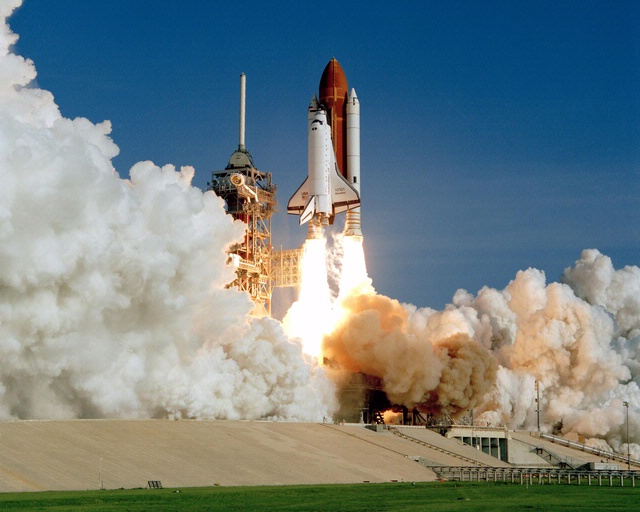
\includegraphics[scale=0.35]{gambar/roketluarangkasa.jpg}

  % Ubah dengan keterangan gambar yang diinginkan
  \caption{Diagram \emph{Fishbone}}
  \label{fig:fishbone}
\end{figure}

\subsection{\emph{Automated Debugging in Data-Intensive Scalable Computing}}
\label{subsec:Automated Debugging in Data-Intensive Scalable Computing}

Penelitian yang dilakukan oleh Muhammad Ali Gulzar dan rekan-rekannya fokus pada pengembangan beban kerja \emph{Big Data Analytics}. Mereka menghadapi tantangan dalam \emph{debugging}, terutama terkait dengan data tidak terstruktur dan asumsi yang salah mengenai data, yang sering menyebabkan kesalahan dalam program. Untuk mengatasi masalah ini, penelitian ini memperkenalkan metode baru yang disebut BIGSIFT, yang berfokus pada menemukan lokasi data yang menyebabkan kegagalan. Metode yang digunakan yaitu menggabungkan isolasi kesalahan otomatis dalam rekayasa perangkat lunak dengan \emph{provenans} data dalam sistem basis data. Hasil dari penelitian ini adalah peningkatan drastis dalam akurasi dalam menentukan lokasi kesalahan, dengan hasil yang lebih akurat hingga ribuan hingga jutaan kali lipat dibandingkan dengan metode sebelumnya seperti provenans data Titian dan \emph{Delta Debugging}. Dengan demikian, penelitian ini berpotensi memberikan manfaat besar dalam mempercepat proses \emph{debugging} pada beban kerja \emph{Big Data Analytics}, sehingga pengembang dapat mengidentifikasi dan memperbaiki masalah lebih efisien.

\subsection{\emph{BigFuzz: Efficient Fuzz Testing for Data Analytics Using Framework Abstraction}}
\label{subsec:BigFuzz: Efficient Fuzz Testing for Data Analytics Using Framework Abstraction}

Dalam penelitian yang dilakukan oleh Qian Zhang dan timnya, mereka mengatasi tantangan dalam pengujian otomatis untuk sistem data-intensive scalable computing (DISC), yang sangat penting untuk menangani kumpulan data besar dalam konteks analisis big data. Masalah utamanya terletak pada kompleksitas intrinsik dari aplikasi berbasis data semacam itu, di mana data seringkali tidak lengkap, terus berubah, dan sulit untuk diprediksi. Pengujian \emph{fuzzing} tradisional, meskipun efektif di domain lain seperti keamanan, menghadapi hambatan yang signifikan ketika diterapkan langsung pada analisis big data. Alasannya termasuk lamanya latensi sistem DISC, tidak praktisnya cakupan cabang konvensional, dan kesulitan dalam menghasilkan data yang bermakna dengan mutasi acak. Untuk mengatasi tantangan ini, para peneliti mengusulkan alat pengujian \emph{fuzzing} yang dipandu cakupan yang baru untuk analisis big data, yang disebut BigFuzz. Alat ini berfokus pada pengujian logika aplikasi daripada peningkatan cakupan kode kerangka kerja, dengan mengabstraksi kerangka kerja DISC menggunakan spesifikasi. BigFuzz juga menggunakan operator \emph{schema-aware data mutation} berdasarkan analisis mendalam tentang jenis kesalahan aplikasi DISC. Hasil penelitian menunjukkan bahwa BigFuzz secara signifikan mempercepat proses \emph{fuzzing}, meningkatkan cakupan kode, dan meningkatkan deteksi kesalahan dalam aplikasi DISC, menjadikannya alat berharga untuk \emph{debugging} beban kerja analisis \emph{big data}, dapat diterapkan pada beragam program, dan mampu menemukan lebih banyak kesalahan dibandingkan dengan pendekatan terkini yang menggunakan eksekusi simbolik.

\subsection{\emph{BigTest: A Symbolic Execution Based Systematic Test Generation Tool for Apache Spark}}
\label{subsec:BigTest: A Symbolic Execution Based Systematic Test Generation Tool for Apache Spark}

Muhammad Ali Gulzar dan timnya melakukan penelitian dalam bidang sistem komputasi berbasis data yang besar (DISC), seperti MapReduce milik Google, Apache Hadoop, dan Apache Spark, yang digunakan luas dalam layanan produksi. Meskipun aplikasi DISC sangat populer, seringkali kualitas aplikasinya kurang baik karena kurangnya pengujian yang menyeluruh dan otomatis. Saat ini, pengujian aplikasi DISC biasanya hanya menggunakan contoh kecil acak dari data masukan, yang mungkin tidak cukup untuk menemukan masalah dalam program. Pengujian aplikasi DISC memiliki tantangan tersendiri karena menggabungkan operasi aliran data dan relasional, serta fungsi yang bisa sangat kompleks.Untuk mengatasi masalah ini, para peneliti memperkenalkan kerangka pengujian putih yang baru bernama BigTest. BigTest digunakan untuk program Apache Spark dan secara otomatis menghasilkan data buatan untuk pengujian yang efektif dan efisien. BigTest menggabungkan eksekusi simbolik fungsi pengguna dengan spesifikasi logis operasi aliran data dan relasional untuk mengeksplorasi semua jalur dalam aplikasi DISC. Hasil eksperimen menunjukkan bahwa BigTest mampu menemukan dua kali lipat lebih banyak masalah daripada menggunakan seluruh dataset dengan waktu pengujian yang jauh lebih singkat (194 kali lebih cepat). BigTest diimplementasikan sebagai alat baris perintah berbasis Java dengan file biner pra-kompilasi. Pengguna dapat menyesuaikan preferensi melalui file konfigurasi, termasuk program target, batasan eksplorasi \emph{loop}, dan pemilihan penyelesaian teorema. Penelitian ini berpotensi meningkatkan pengujian aplikasi DISC, sehingga masalah dalam program dapat ditemukan dengan lebih efektif dan efisien.

\subsection{\emph{Titian: Data Provenance Support in Spark}}
\label{subsec:Titian: Data Provenance Support in Spark}

Matteo Itterlandi dan timnya mengatasi tantangan yang sulit dalam melakukan \emph{debugging} pada logika pemrosesan data di dalam sistem Data-Intensive Scalable Computing (DISC). Biasanya, \emph{debugging} dalam sistem ini memakan banyak waktu dan usaha karena kurangnya alat \emph{debugging} yang memadai, seringkali memerlukan pengumpulan bukti secara manual dari file log dan mencoba-coba. Untuk mempermudah proses ini, mereka mengembangkan Titian, sebuah perpustakaan yang memungkinkan pelacakan asal data - mengikuti jejak data melalui berbagai transformasi di Apache Spark. Dengan menggunakan ekstensi Spark Titian, ilmuwan data dapat dengan cepat mengidentifikasi data masukan yang menjadi penyebab potensial kesalahan atau hasil yang tidak biasa. Titian terintegrasi dengan baik ke dalam \emph{platform} Spark dan menyediakan dukungan asal data dengan kecepatan interaktif, jauh lebih cepat dibandingkan dengan solusi yang sudah ada, dengan dampak minimal pada kinerja pekerjaan Spark. \emph{Overhead} untuk mengambil jejak data biasanya tidak lebih dari 30\% dari waktu eksekusi pekerjaan dasar. Penelitian ini secara signifikan meningkatkan efisiensi dalam \emph{debugging} logika pemrosesan data dalam sistem DISC, memberikan pendekatan yang lebih efektif dan menghemat waktu bagi ilmuwan data dalam mengidentifikasi dan memecahkan masalah.

\subsection{\emph{Automatic Romanian Text Generation Using GPT-2}}
\label{subsec:Automatic Romanian Text Generation Using GPT-2}

Marius Cristian Buzea dan timnya melakukan penelitian di bidang pemrosesan bahasa alami (NLP), khususnya dalam menghasilkan teks. Mereka menggunakan model transformer besar yang sudah dilatih sebelumnya seperti GPT-2 dan GPT-3 dari OpenAI, serta BERT dari Google. Penelitian ini mengembangkan model NLG berbasis arsitektur GPT-2 untuk menghasilkan teks dalam bahasa Rumania dengan menggunakan teks yang dianotasi secara manual. Model kecil GPT-2 Rumania, bernama MCBGPT-2, dilatih dan diuji dengan 24 ribu berita. Selain itu, model GPT-2 Rumania yang ada, RoGPT-2, juga digunakan dalam eksperimen. Evaluasi menggunakan metrik otomatis seperti BLEU, ROUGE, BLEURT, dan BERTScore menunjukkan bahwa model MCBGPT-2 dan RoGPT-2 memiliki kinerja yang serupa dalam tugas penghasil teks untuk bahasa Rumania, dengan MCBGPT-2 memerlukan lebih sedikit data untuk proses pelatihannya. Hasil eksperimen menunjukkan bahwa MCBGPT-2 dan RoGPT-2 memberikan kinerja yang hampir sama dalam menghasilkan teks dalam bahasa Rumania, namun MCBGPT-2 memerlukan lebih sedikit data selama pelatihan. Selain itu, arsitektur transformer yang digunakan oleh GPT-2 memungkinkan kecepatan pelatihan yang lebih tinggi dan kemampuan paralelisasi yang lebih baik. Penelitian ini menyimpulkan bahwa model MCBGPT-2 adalah alternatif yang efisien untuk model RoGPT-2 yang ada, terutama dalam menghasilkan kalimat panjang menggunakan data pelatihan yang lebih sedikit.

\section{Dasar Teori}
\label{sec:dasarTeori}

Pada subbab ini akan dijelaskan dasar teori yang digunakan dalam penelitian ini. Berdasarkan pada subbab 2.1, penelitian ini akan diterapkan pada sistem Data-Intensive Scalable Computing (DISC). DISC itu sendiri merupakan pendekatan komputasi yang terfokus pada pengolahan dan analisis data dalam skala besar di mana tujuan utamanya adalah memastikan bahwa data ini dapat digunakan untuk mendapatkan wawasan berharga, mendukung pengambilan keputusan, dan mengidentifikasi pola yang relevan dalam data tersebut [8]. Hingga saat ini, telah banyak platform yang dibangun untuk dapat memonitoring proses kerja sistem DISC [9].

Sistem DISC ini akan dibangun menggunakan Apache Spark, yaitu sebuah platform pemrosesan data open source yang sangat kuat dan populer. Dirancang untuk mengatasi tantangan pemrosesan data dalam skala besar, Spark menyediakan kerangka kerja yang efisien untuk mengelola dan menganalisis data dalam volume besar dengan kecepatan tinggi. Salah satu fitur utama dari Spark adalah kemampuannya untuk menggabungkan pemrosesan batch dan pemrosesan aliran data dalam satu framework yang kuat, yang memungkinkan pengguna untuk melakukan analisis data real-time dan batch dengan efisiensi tinggi. Spark juga mendukung pemrosesan data terdistribusi dan pemrosesan paralel, yang membuatnya sangat cocok untuk tugas-tugas yang membutuhkan komputasi tingkat tinggi. Ini memiliki antarmuka pemrograman yang beragam, termasuk Python, Scala, dan Java, sehingga dapat diakses oleh berbagai pengembang. Spark juga memiliki perpustakaan yang kaya, seperti MLib untuk pembelajaran mesin, SQL untuk kueri data, dan Streaming untuk pemrosesan aliran data [10]. Platform ini telah menjadi pilihan populer dalam berbagai industri, termasuk analisis data, ilmu data, dan pemrosesan aliran data [11]. 

Untuk dapat memisahkan antara data benar dan data yang bermasalah akan digunakan sebuah library bernama Spark Titian. Spark Titian merupakan sebuah perpustakaan yang dirancang untuk memungkinkan provenans data interaktif dalam lingkungan Apache Spark. Titian terintegrasi dengan antarmuka pemrograman Spark, yang berdasarkan abstraksi Resilient Distributed Dataset (RDD) yang menentukan serangkaian transformasi dan tindakan untuk memproses kumpulan data. Data yang dihasilkan dari serangkaian transformasi tertentu yang menghasilkan RDD dapat disimpan dalam memori. Spark menjaga sejarah transformasi program sehingga dapat memulihkan partisi RDD yang hilang dalam kasus kegagalan. Titian memperkaya abstraksi RDD dengan kemampuan provenans data yang sangat terinci. Ini memungkinkan seorang pemrogram Spark untuk mengakses referensi LineageRDD dari RDD tertentu, memfasilitasi fungsionalitas pelacakan data, yaitu kemampuan untuk berpindah mundur (atau maju) dalam aliran data program Spark. Dari referensi LineageRDD tertentu, yang sesuai dengan posisi dalam eksekusi program, dapat memanggil transformasi RDD asli apa pun, menghasilkan RDD baru yang memproses subset data yang dirujuk oleh LineageRDD. Kemampuan ini menyederhanakan kemampuan untuk melacak baik ke belakang maupun ke depan dalam aliran data, memungkinkan eksekusi serangkaian transformasi RDD asli baru pada data yang dirujuk. Dukungan pelacakan yang disediakan oleh LineageRDD terintegrasi dengan operator batch internal Spark dan mekanisme toleransi kesalahan. Akibatnya, Titian dapat digunakan dalam sesi terminal Spark, menyediakan dukungan provenans data interaktif bersama dengan kueri ad-hoc Spark asli [7].

Selain itu, untuk dapat mengganti data yang bermasalah dengan data yang benar, akan digunakan sebuah model yang disediakan oleh HugginFace. HuggingFace adalah sebuah perusahaan yang dikenal sebagai pemimpin dalam bidang pemrosesan bahasa alami (Natural Language Processing, NLP). Misi inti mereka adalah membuat teknologi NLP yang kuat dan canggih lebih mudah diakses oleh para peneliti, ilmuwan data, pengembang, dan perusahaan [12]. Salah satu kontribusi utama HuggingFace adalah penyediaan berbagai model NLP "state-of-the-art" yang telah dilatih dengan data besar, seperti model BERT, DistilBert, GPT-2, DistilGPT2, dan banyak lagi. Model-model ini sangat kuat dan dapat digunakan dalam berbagai tugas, seperti penerjemahan bahasa, analisis sentimen, generate teks otomatis, dan pemahaman bahasa alami [13]. Selain itu, HuggingFace juga menyediakan API yang mempermudah penggunaan model NLP tersebut. Mereka juga mengembangkan alat-alat dan perpustakaan (library) yang mendukung pengembangan dan penelitian di bidang NLP [14]. Dengan demikian, HuggingFace berperan penting dalam memperluas akses ke teknologi NLP canggih, memungkinkan inovasi di berbagai industri, termasuk pemrosesan teks, layanan pelanggan, penelitian akademik, dan banyak lagi [15].

DistilGPT2 Model dipilih sebagai model yang akan digunakan pada penelitian ini. DistilGPT2 adalah model NLP yang dikembangkan oleh HuggingFace, yang merupakan versi ringan (distil) dari model GPT-2 (Generative Pre-trained Transformer 2). Keunggulan DistilGPT2 terletak pada efisiensi komputasi, membuatnya sangat cocok untuk aplikasi yang membutuhkan pemrosesan teks cepat dalam skala besar. DistilGPT2 mempertahankan arsitektur dasar GPT-2 dengan lapisan dan parameter lebih sedikit, membuatnya lebih ringan dan cepat. Meskipun lebih kecil, DistilGPT2 mampu menghasilkan teks dengan baik dan cocok untuk aplikasi NLP pada perangkat dengan sumber daya terbatas. Hasil evaluasi menunjukkan bahwa DistilGPT2 memiliki performa yang kompetitif dan efisien. Hal ini membuat DistilGPT2 menjadi pilihan yang menarik dalam pengembangan aplikasi yang bergantung pada analisis teks dengan kecepatan dan efisiensi [6].

Untuk dapat menghubungkan antara DistilGPT2 Model dan program DISC yang menggunakan Titian, penelitian ini akan memanfaatkan FastAPI. FastAPI adalah kerangka kerja web Python yang dikenal dengan kinerja tinggi, kemudahan pengembangan, dan otomatisasi pembuatan dokumentasi API. Dibangun di atas Python 3.6+ yang mendukung asynchronous programming, FastAPI dapat menangani banyak permintaan dengan cepat. Kerangka kerja ini menggunakan teknologi seperti Starlette dan Pydantic untuk memastikan penanganan permintaan HTTP yang efisien dan validasi data yang kuat [17]. Hingga kini FastAPI telah banyak dimanfaatkan untuk keperluan machine learning dan data science dan terbukti 45% jauh lebih baik dibandingkan dengan Flask [18]. Flask adalah framework web Python yang ringan dan fleksibel yang menekankan kesederhanaan dan kemampuan untuk diperluas. Ini menyediakan fitur dasar untuk pengembangan web dan memungkinkan pengembang memilih dan mengintegrasikan ekstensi berdasarkan kebutuhan proyek mereka [19].

DistilGPT2 Model yang ditanamkan ke dalam FastAPI kemudian akan di-deploy menggunakan Amazon Web Service (AWS) EC2. AWS adalah platform komputasi awan yang dikelola oleh Amazon. AWS menyediakan berbagai layanan komputasi, penyimpanan, database, jaringan, dan lainnya yang dapat digunakan oleh perusahaan dan pengembang untuk menjalankan aplikasi mereka di lingkungan awan. Amazon EC2 adalah salah satu layanan inti di AWS yang memungkinkan pengguna untuk menyewa mesin virtual (instance) di cloud. Pengguna dapat memilih berbagai jenis instance yang sesuai dengan kebutuhan mereka, seperti instance berkinerja tinggi, instance berbasis GPU, atau instance berbiaya rendah. AWS EC2 memungkinkan pengguna untuk dengan cepat meluncurkan, mengelola, dan menghentikan instance sesuai kebutuhan, sehingga mereka dapat mengskalakan aplikasi mereka sesuai dengan permintaan dan menghemat biaya saat instance tidak digunakan [20]. Dibandingkan dengan kompetitornya, AWS EC2 menawarkan solusi yang lebih baik di mana pengguna dapat memiliki kesempatan untuk memilih fitur yang diinginkan sesuai kebutuhan [21]. 

Pengembangan sistem akan menggunakan 2 bahasa pemrograman. Pada proses training awal model dan pembuatan FastAPI, bahasa pemrograman yang akan digunakan adalah Python. Sedangkan pada pembuatan sistem yang akan mengonsumsi FastAPI, bahasa pemrograman yang akan digunakan adalah Scala. Python dipilih untuk proses training awal model dan pembuatan FastAPI karena memiliki sintaksis yang mudah dipahami, ekosistem yang kaya, serta banyak library dan framework yang mendukung pengembangan aplikasi machine learning dan web termasuk HuggingFace. Kelebihan Python dalam kesederhanaan dan kemudahan penggunaan membuatnya menjadi pilihan utama dalam fase awal pengembangan [22]. Sementara itu, Scala dipilih untuk pembuatan sistem yang mengonsumsi FastAPI karena Scala menawarkan keunggulan dalam hal konkurensi dan eksekusi paralel, yang dapat meningkatkan kinerja sistem secara signifikan. Pemilihan Scala juga didorong oleh keandalan dan ekosistem yang mapan, terutama dalam pengembangan aplikasi berukuran besar [23]. Dibandingkan dengan Java pada bidang Natural Language Processing (NLP), Scala dianggap lebih unggul karena ekosistemnya yang lebih modern dan fitur-fitur fungsional yang dapat mempermudah pengembangan aplikasi NLP [24]. Scala memungkinkan penggunaan paradigma fungsional yang mendukung pemrosesan data kompleks dan manipulasi struktur data dengan lebih efisien, sehingga menjadi pilihan yang tepat untuk tugas-tugas kompleks dalam NLP [25].

\cleardoublepage

% Bab 3 desain dan implementasi
\chapter{DESAIN DAN IMPLEMENTASI}
\label{chap:desainimplementasi}

% Ubah bagian-bagian berikut dengan isi dari desain dan implementasi

Penelitian ini dilaksanakan sesuai \lipsum[1][1-5]

\section{Deskripsi Sistem}
\label{sec:deskripsisistem}

Sistem akan dibuat dengan \lipsum[1-2]

\section{Implementasi Alat
  \label{sec:implementasi alat}}

Alat diimplementasikan dengan \lipsum[1]

% Contoh pembuatan potongan kode
\begin{lstlisting}[
  language=C++,
  caption={Program halo dunia.},
  label={lst:halodunia}
]
#include <iostream>

int main() {
    std::cout << "Halo Dunia!";
    return 0;
}
\end{lstlisting}

\lipsum[2-3]

% Contoh input potongan kode dari file
\lstinputlisting[
  language=Python,
  caption={Program perhitungan bilangan prima.},
  label={lst:bilanganprima}
]{program/bilangan-prima.py}

\lipsum[4]

\cleardoublepage

% Bab 4 pengujian dan analisis
\chapter{PENGUJIAN DAN ANALISIS}
\label{chap:pengujiananalisis}

% Ubah bagian-bagian berikut dengan isi dari pengujian dan analisis

Pada penelitian ini dipaparkan \lipsum[1][1-5]

\section{Skenario Pengujian}
\label{sec:skenariopengujian}

Pengujian dilakukan dengan \lipsum[1-2]

\section{Evaluasi Pengujian}
\label{sec:analisispengujian}

Dari pengujian yang \lipsum[1]

% Contoh pembuatan tabel
\begin{longtable}{|c|c|c|}
  \caption{Hasil Pengukuran Energi dan Kecepatan}
  \label{tb:EnergiKecepatan}                                   \\
  \hline
  \rowcolor[HTML]{C0C0C0}
  \textbf{Energi} & \textbf{Jarak Tempuh} & \textbf{Kecepatan} \\
  \hline
  10 J            & 1000 M                & 200 M/s            \\
  20 J            & 2000 M                & 400 M/s            \\
  30 J            & 4000 M                & 800 M/s            \\
  40 J            & 8000 M                & 1600 M/s           \\
  \hline
\end{longtable}

\lipsum[2-4]

\cleardoublepage

% Bab 5 penutup
\chapter{PENUTUP}
\label{chap:penutup}

% Ubah bagian-bagian berikut dengan isi dari penutup

\section{Kesimpulan}
\label{sec:kesimpulan}

Berdasarkan hasil pengujian yang \lipsum[1][1-3] sebagai berikut:

\begin{enumerate}[nolistsep]

  \item Pembuatan \lipsum[2][1-3]

  \item \lipsum[2][4-6]

  \item \lipsum[2][7-10]

\end{enumerate}

\section{Saran}
\label{chap:saran}

Untuk pengembangan lebih lanjut pada \lipsum[1][1-3] antara lain:

\begin{enumerate}[nolistsep]

  \item Memperbaiki \lipsum[2][1-3]

  \item \lipsum[2][4-6]

  \item \lipsum[2][7-10]

\end{enumerate}

\cleardoublepage

\chapter*{DAFTAR PUSTAKA}
\addcontentsline{toc}{chapter}{DAFTAR PUSTAKA}
\renewcommand\refname{}
\vspace{2ex}
\renewcommand{\bibname}{}
\begingroup
\def\chapter*#1{}
\printbibliography
\endgroup
\cleardoublepage

% Biografi penulis
\begin{center}
  \Large
  \textbf{BIOGRAFI PENULIS}
\end{center}

\addcontentsline{toc}{chapter}{BIOGRAFI PENULIS}

\vspace{2ex}

\begin{wrapfigure}{L}{0.3\textwidth}
  \centering
  \vspace{-3ex}
  % Ubah file gambar berikut dengan file foto dari mahasiswa
  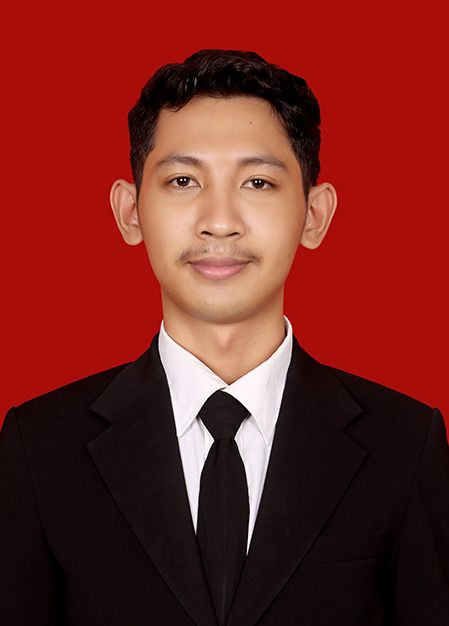
\includegraphics[width=0.3\textwidth]{gambar/jabalnur.jpeg}
  \vspace{-4ex}
\end{wrapfigure}

% Ubah kalimat berikut dengan biografi dari mahasiswa
\name{}, dilahirkan di Pangkep, 29 Juni 2000, merupakan anak pertama dan terakhir
dari kedua orang tuanya. Penulis telah menyelesaikan pendidikan di SDN 14 Bonto Tene, 
SMPN 2 Pangkep, SMAN 11 Pangkep, dan S1 Teknik Informatika Universitas Hasanuddin. Pada
tahun 2020, penulis mengikuti SBMPTN dan diterima di Institut Teknologi Sepuluh Nopember
pada program studi S1 \department{} Fakultas \facultyshort{} \institute{} dengan NRP 5025201241.

Di departemen \department{}, penulis aktif dalam berbagai kegiatan organisasi 
dan kepanitiaan. Penulis sempat menjabat sebagai Wakil Ketua Himpunan Eksternal
Departemen Teknik Informatika pada tahun 2023. Penulis dapat dihubungi melalui 
email \href{mailto:\email}{\email}.


\cleardoublepage

\end{document}
